\documentclass{article}


\usepackage{arxiv}

\usepackage[utf8]{inputenc} % allow utf-8 input
\usepackage[T1]{fontenc}    % use 8-bit T1 fonts
\usepackage{hyperref}       % hyperlinks
\usepackage{url}            % simple URL typesetting
\usepackage{booktabs}       % professional-quality tables
\usepackage{amsfonts}       % blackboard math symbols
\usepackage{nicefrac}       % compact symbols for 1/2, etc.
\usepackage{microtype}      % microtypography
\usepackage{graphicx}
\usepackage{natbib}
\usepackage{doi}

\usepackage{amsmath}
\usepackage{nicematrix}
\usepackage{cleveref}
\usepackage{listings}
\usepackage{pgfplots}


\NiceMatrixOptions{cell-space-top-limit=5pt,cell-space-bottom-limit=5pt,columns-width=20pt}

\crefname{lstlisting}{listing}{listings}
\Crefname{lstlisting}{Listing}{Listings}


% Listing options
\definecolor{codegreen}{rgb}{0,0.6,0}
\definecolor{codegray}{rgb}{0.5,0.5,0.5}
\definecolor{codepurple}{rgb}{0.58,0,0.82}
\definecolor{backcolour}{rgb}{0.95,0.95,0.92}

\lstdefinestyle{python_style}{
    backgroundcolor=\color{backcolour},
    commentstyle=\color{codegreen},
    keywordstyle=\color{magenta},
    numberstyle=\tiny\color{codegray},
    stringstyle=\color{codepurple},
    basicstyle=\ttfamily\footnotesize,
    breakatwhitespace=false,
    breaklines=true,
    captionpos=b,
    keepspaces=true,
    numbers=left,
    numbersep=5pt,
    showspaces=false,
    showstringspaces=false,
    showtabs=false,
    tabsize=2
}
\lstset{style=python_style}


\newcommand{\irow}[1]{% inline row vector
  {\begin{smallmatrix}(\,#1\,)\end{smallmatrix}}^T
}


\def\R{\mathbb{R}}
\def\xt{\tilde{x}}


\title{Linear programming project}

%\date{September 9, 1985}	% Here you can change the date presented in the paper title
\date{} 					% Or removing it

\author{
  \hspace{1mm}Dmitry Beresnev \\
	AIDS-MS1, Innopolis University\\
	\texttt{d.beresnev@innopolis.university} \\
	\And{}
  \hspace{1mm}Vsevolod Klyushev \\
	AIDS-MS1, Innopolis University\\
	\texttt{v.klyushev@innopolis.university}
}

\renewcommand{\undertitle}{\textbf{Group 2} Report for Optimization F24 course}
\renewcommand{\headeright}{}

\begin{document}
\maketitle


\section{Introduction}
Initial problem is formulated as following:
\begin{equation}\label{eq:init}
  \begin{aligned}
                 & \min\limits_{x' \in \R^p} {\| Ax'-y' \|}_1 \\
    \text{s.t. } & 0 \leq x' \leq 1
  \end{aligned}
\end{equation}
where $A \in \R^{m \times p}$ with $m \geq p$ --- message  encoding matrix,
$y'$ --- received encoded (noisy) message,
$x'$ --- encoded initial message to be found.

\section{Notations}

 {
  \renewcommand{\arraystretch}{1.5}
  \renewcommand{\tabcolsep}{10pt}
  \begin{table}[hbthbt]
    \centering
    \begin{tabular}{cc}
      \toprule
      \textbf{Notation}                          & \textbf{Meaning}                                     \\
      \midrule
      $e_i$                                      & unit vector with 1 at index $i$ and all other zeroes \\
      $1_n$                                      & vector of $n$ ones                                   \\
      $I_n$                                      & identity matrix of size $n \times n$                 \\
      $0_n$                                      & vector of $n$ zeroes                                 \\
      $0_{m \times n}$                           & zero matrix of size $m \times n$                     \\
      $x_i$ $\left( \text{or } {(Ax)}_i \right)$ & $i$-th component of vector $x$    (or $Ax$)          \\

      \bottomrule
    \end{tabular}
  \end{table}
 }


\section{Q1: Linear problem formulation}
Initial problem (\cref{eq:init}) is not linear as cost function
$ {\| Ax'-y' \|}_1 = \sum_{i=1}^{m} |{(Ax')}_i-y'_i|$, is not linear. However, this objective function is \textbf{piecewise linear convex} function. Therefore, each element $|{(Ax')}_i-y'_i| = \max({(Ax')}_i-y'_i, y'_i -{(Ax')}_i)$ can be substituted with new variable $z'$ with the following additional
constraints: $z_i \geq {(Ax')}_i-y'_i$ and $z_i \geq y'_i-{(Ax')}_i$.

So the following problem is \textbf{linear} and is equivalent to the initial one:
\begin{equation}\label{eq:linear}
  \begin{aligned}
                 & \min\limits_{x' \in \R^p, z \in \R^m} \sum_{i=1}^{m} z_i \\
    \text{s.t. } & x' \geq 0                                                \\
                 & x' \leq 1                                                \\
                 & z_i \geq {(Ax')}_i-y'_i, \ i = 1 \dots m                 \\
                 & z_i \geq y'_i-{(Ax')}_i, \ i = 1 \dots m                 \\
  \end{aligned}
\end{equation}

\section{Q2: Linear problem in standard form}

For the easier and more evident derivation of standard form of \Cref{eq:linear},
linear problem will be firstly rewritten in geometric form, and only then --- in standard. The obtained linear optimization problem in standard form will be equivalent to initial problem (\cref{eq:init}).

\subsection{Geometric form}\label{sec:geom}

The equivalent \textbf{geometric} form of \Cref{eq:linear} is
\begin{equation}\label{eq:geom}
  \begin{aligned}
                 & \min\limits_{z' \in \R^{p+m}} c^T z' \\
    \text{s.t. } &
    \begin{pNiceArray}{c:c}
      I_p  & 0_{p \times m}  \\
      \hdottedline
      -I_p  & 0_{p \times m}  \\
      \hdottedline
      -A & I_m \\
      \hdottedline
      A & I_m \\
      \CodeAfter
      \UnderBrace[yshift=1.5mm,color=blue]{last-1}{last-last}{A'}
    \end{pNiceArray}
    z' \geq
    \begin{pNiceMatrix}
      0_p  \\
      -1_p \\
      -y'  \\
      y'   \\
      \CodeAfter
      \UnderBrace[yshift=1.5mm,color=blue]{last-1}{last-last}{b'}
    \end{pNiceMatrix},
  \end{aligned}
  \vspace{20pt}
\end{equation}
where
$c = \sum_{i=p+1}^{p+m} e_i \in \R^{(p+m)}$,
$b' \in \R^{2p+2m}$ and
$A'\in \R^{(2p+2m) \times (p+m)}$.

The first $p$ components of $z'$ correspond to the components of $x'$, and the next $m$ components correspond to the components of $z$ from \Cref{eq:linear}. Rows and columns of $A'$ representation in \Cref{eq:geom} are separated in blocks for clarity: the vertical separation is for $x'$ and $z$ correspondingly, and the horizontal separations denote corresponding constraints from \Cref{eq:linear}.

\subsection{Standard form}\label{sec:std}

Note that $z' = {(x', z)}^T$ from \Cref{eq:geom} is already non-negative, because $x' \geq 0$ by problem definition and $z \geq 0 $ by construction\footnote{Intuitively, $z$ substitutes the absolute value, so is non-negative. Formally, from \Cref{eq:linear}, $z \geq t$ and $z \geq -t$ for some $t$. So if $t \geq 0$, then $z \geq t \geq 0$, and if $t \leq 0$ then $z \geq -t \geq 0$ }. Therefore, to convert \Cref{eq:geom} to standard form, only introduction of slack variables is needed to get rid of inequality sign. The equivalent \textbf{standard} form of \Cref{eq:geom} is
\begin{equation}\label{eq:std}
  \begin{aligned}
                 & \min\limits_{\xt \in \R^{2p+3m}} c^T \xt    \\
    \text{s.t. } &
    \begin{pNiceArray}{c:c:c}
      -I_p  & 0_{p \times m} &  \\
      \Hdotsfor{2} & \\
      -A & I_m & -I_{p+2m}\\
      \Hdotsfor{2} & \\
      A & I_m & \\
      \CodeAfter
      \UnderBrace[yshift=1.5mm,color=blue]{last-1}{last-last}{A'}
    \end{pNiceArray}
    \xt =
    \begin{pNiceMatrix}
      -1_p \\
      -y'  \\
      y'   \\
      \CodeAfter
      \UnderBrace[yshift=1.5mm,color=blue]{last-1}{last-last}{b'}
    \end{pNiceMatrix}, \\
    \vspace{20pt}                                              \\
                 & \xt \geq 0,
  \end{aligned}
  \vspace{20pt}
\end{equation}
where
$c = \sum_{i=p+1}^{p+m} e_i \in \R^{(2p+3m)}$,
$b' \in \R^{p+2m}$
and $A'\in \R^{(p+2m) \times (2p+3m)}$. Here, $-I_{p+2m}$ represents necessary slack variables.

The first $p$ components of $\xt$ correspond to the components of $x'$, the next $m$ components correspond to the components of $z$ from \Cref{eq:linear} and the last $(p+2m)$ components correspond to slack variables $s$. Rows and columns of $A'$ representation in \Cref{eq:std} are again separated in blocks for clarity: the vertical separations are for $x'$, $z$ and $s$ correspondingly, and the horizontal separations are related to corresponding constraints from \Cref{eq:geom} (except first one, as non-negativity in standard from is separate constraint).

% Hereafter, if other is not mentioned, the mentions of $c$, $A'$ and $b'$ are referred to the \Cref{eq:std}.

\section{Q3: Message decryption}

In the sake of research interest, the message decrypted by solving three different problems: the least squares (assuming no noise at all), linear optimization program (LOP) in geometric form and linear optimization problem in standard form.

\subsection{Least Squares}
As it is previously mentioned, this approach is quite naive as assumes no noise in received signal $y'$. The function \textit{scipy.linalg.lstsq} is used, so the encoded message is found as a solution to the problem $\min\limits_{x' \in \R^p} {\| Ax'-y' \|}_2$. The resulting function is demonstrated on \Cref{lst:naive}.


\subsection{LOP in geometric form}
In this case, the encoded message is found as a solution to the problem \Cref{eq:geom} using the function \textit{scipy.optimize.linprog}. The resulting function is demonstrated on \Cref{lst:geom}. As one can notice, the construction of $A$ and $b$ completely reflects representations of $A'$ and $b'$ from \Cref{eq:geom}. Also, as was mentioned in \Cref{sec:geom}, we are interested only in the first $p$ components of the solution.


\subsection{LOP in standard form}
The encoded message is found as a solution to the problem \Cref{eq:std} using the function \textit{scipy.optimize.linprog}. The resulting function is demonstrated on \Cref{lst:std}. As one can notice, the construction of $A$ and $b$ completely reflects representations of $A'$ and $b'$ from \Cref{eq:std}.
Also, as was mentioned in \Cref{sec:std}, we are interested only in the first $p$ components of the solution.



\subsection{Results}
As expected, result of naive solution is a total mess, while the solution of LOP of both forms led to meaningful message:

\begin{equation*}
  \begin{aligned}
    \textbf{You can claim your personal reward by going to Student affairs, giving you code=1083 and ask for you reward}
  \end{aligned}
\end{equation*}

Also note that computation time of standard LOP (334 seconds) is 14\% greater than of geometric LOP (293 seconds)\footnote{Possible explanation is that standard LOP has bigger dimension of target vector than geometric LOP. Namely, as in given case $p=856, m=4p=3424$, $\xt$ from \Cref{eq:std} is from $\R^{14p} = \R^{11984}$ while $z'$ from \Cref{eq:geom} is only from $\R^{5p} = \R^{4280}$.
}.


\section{Q4: Check if the obtained solution is a polyhedron vertex}

In this section the linear program in geometric form is considered, as the verifying that the point is
a vertex of polyhedron in geometric form is easier than in case of polyhedron in standard form.

For polyhedron in geometric form, the following is true: for the feasible solution $x \in \R^n$, if polyhedron has $n$ linearly independent constraints active (or tight) at $x$, then $x$ --- vertex of this polyhedron.
For polyhedron defined in \Cref{eq:geom}, it is needed to verify that there are $(p+m)$ tight linearly independent constraints $A' z^\ast \geq b'$, where $z^\ast \in \R^{p+m}$ --- solution of linear problem in geometric form obtained with \Cref{lst:geom}.

Using code snippet presenting on \Cref{lst:vertex}, we determined that obtained solution $z^\ast$ is indeed vertex of polyhedron in geometric form: there are exactly $(p+m)$ linearly independent constraints (what means that vertex even is not degenerate). Note that \textit{np.isclose()} function is used as Python language can not guarantee numeric precision of values close to zero, so values like $10^{-10}$ should be indeed treated as 0.

\section{Q5: Custom message experiments}

To determine maximum level of noise up to what the message can be decrypted, the binary search algorithm was used (\Cref{lst:bin}). The maximum level of noise was calculated for three messages of different sizes.  In addition to message length, the \textbf{signal dimension factor} --- the scalar $k$ in equation $m=kp$ for encoding matrix $A \in \R^{m \times p}$ (in initial problem we are given $m=4p$).


The results (\Cref{fig:noise}) are not surprising. The bigger signal dimension factor is the larger the decoded encoded message is, so the message transfer should be more robust to the noise. For example, even with signal dimension factor equals 1, considered messages can be transferred with about 10--20\% disturbed data.


\begin{figure}[hbthbt]
  \centering
  \pgfplotsset{compat=1.10}
  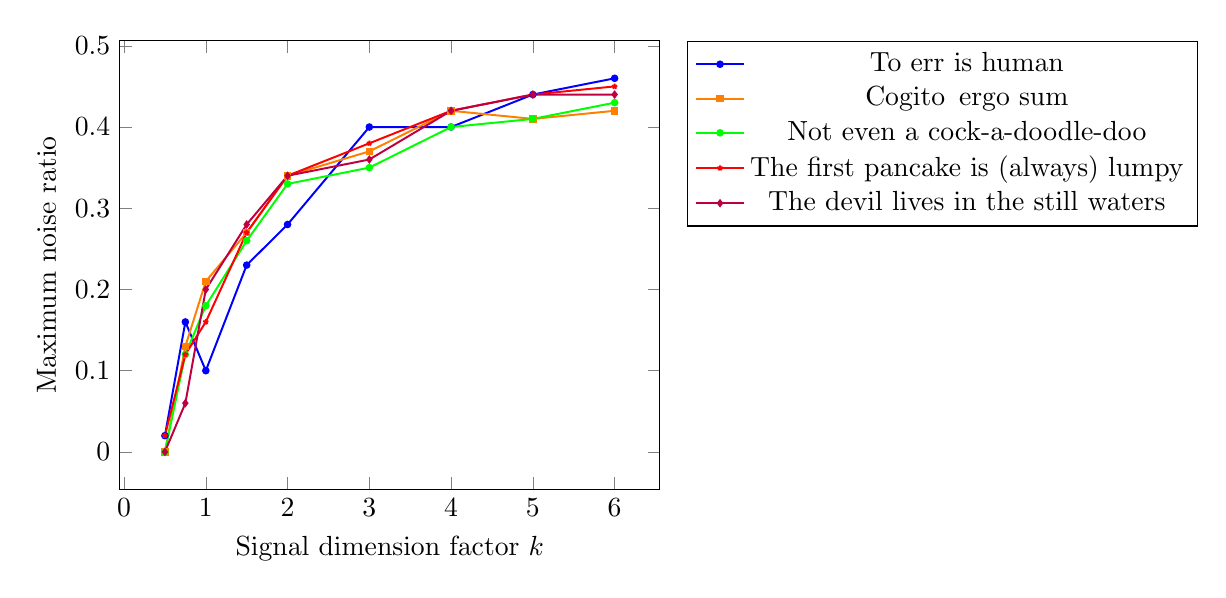
\begin{tikzpicture}
    \begin{axis}[
        legend style={
            at={(1.05,1.0)},
            anchor=north west,
            legend columns=1},
        xlabel = Signal dimension factor $k$,
        ylabel = Maximum noise ratio,
      ]
      \addplot+[sharp plot,mark size=1pt,blue,mark options={fill=blue},line width=0.25mm] coordinates
        {(0.5, 0.02) (0.75, 0.16) (1, 0.1) (1.5, 0.23) (2, 0.28) (3, 0.4) (4, 0.4) (5, 0.44) (6, 0.46)};

      \addplot+[sharp plot,orange,mark size=1pt,mark options={fill=orange},line width=0.25mm] coordinates
        {(0.5, 0.0) (0.75, 0.13) (1, 0.21) (1.5, 0.27) (2, 0.34) (3, 0.37) (4, 0.42) (5, 0.41) (6, 0.42)};

      \addplot+[sharp plot,green,mark size=1pt,mark options={fill=green},line width=0.25mm] coordinates
        {(0.5, 0.0) (0.75, 0.12) (1, 0.18) (1.5, 0.26) (2, 0.33) (3, 0.35) (4, 0.4) (5, 0.41) (6, 0.43)};

      \addplot+[sharp plot,red,mark size=1pt,mark options={fill=red},line width=0.25mm] coordinates
        {(0.5, 0.02) (0.75, 0.12) (1, 0.16) (1.5, 0.27) (2, 0.34) (3, 0.38) (4, 0.42) (5, 0.44) (6, 0.45)};

      \addplot+[sharp plot,purple,mark size=1pt,mark options={fill=purple},line width=0.25mm] coordinates
        {(0.5, 0.0) (0.75, 0.06) (1, 0.2) (1.5, 0.28) (2, 0.34) (3, 0.36) (4, 0.42) (5, 0.44) (6, 0.44)};

      \legend{To err is human,Cogito\, ergo sum,Not even a cock-a-doodle-doo,
        The first pancake is (always) lumpy,The devil lives in the still waters}
    \end{axis}
  \end{tikzpicture}
  \caption[Maximum level of noise up to what the messages can be decrypted]
  {Maximum level of noise up to what the messages can be decrypted.
    Signal dimension factor $k$ is defined from equation $m=kp$ for encoding matrix $A \in \R^{m \times p}$}\label{fig:noise}
\end{figure}


\section{Q6: Dikin's method}

To start the Dikin's method, we first need to get a point from the feasible set of our problem. Since the dimension of our problem is quite large, we decided to use the `dirty' method of getting the starting point. To do this, we had to solve the following problem in a standard form (from lecture slides):

\begin{equation}\label{eq:dikin_init}
  \begin{aligned}
                 & \min\limits_{\xt \in \R^{2p+3m}} 0 \\
    \text{s.t. } & A' \tilde{x} = b                   \\
    \vspace{20pt}                                     \\
                 & \xt \geq \varepsilon,
  \end{aligned}
  \vspace{20pt}
\end{equation}
where $c \in \mathbb{R}^{2p+3m} = 0_{2p+3m} $,
$\varepsilon > 0$ --- small constant ($\varepsilon = 0.00001$ in our experiments),
and other notations are the same as in \Cref{eq:std}. The code with solution of this problem is presented in \Cref{lst:dikin_init}.

Implementation of Dikin's algorithm is demonstrated on \Cref{lst:dikin}. During experiments with message `\textit{I like Jubilee cookies!}' and signal dimension factor $k=2$ and percent of noise in signal 20\%, Dikin's algorithm showed convergence (\cref{fig:dik_single}), and after 538 iterations it was able to fully recover initial message. The overall time taken by algorithm was about 92 seconds. Therefore, the Dikin's algorithm is applicable for message decoding.

However, Dikin's method has several disadvantages. Firstly, it is very sensitive to initial point. Secondly, in comparison to other methods, Dikin's requires more computation time and resources. Thirdly, SciPy solvers do not require initial point in feasible set to start and are more robust, since they support about 36\% noise level, when Dikin's method can handle only about 27\% (\cref{fig:dik_multiple}). Finally, the Dikin's method does not work with linear problem which contains degenerate vertices\footnote{According to Professor Leplat, whom we trust}.

In conclusion, SciPy approaches (\Cref{lst:geom,lst:std}) look more preferable (at least for the given problem).

\begin{figure}[hbthbt]
  \centering
  \pgfplotsset{compat=1.10}
  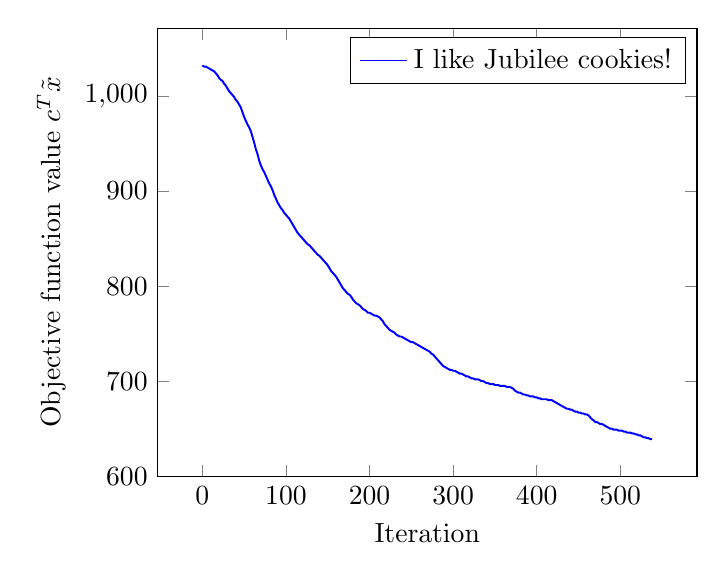
\begin{tikzpicture}
    \begin{axis}[
        xlabel = Iteration,
        ylabel = Objective function value $c^T \xt$
      ]
      \addplot+[mark=none,line width=0.25mm] coordinates
        {(0, 1032) (2, 1031) (4, 1031) (6, 1030) (8, 1029) (10, 1028) (12, 1027) (14, 1026) (16, 1024) (18, 1022) (20, 1019) (22, 1017) (24, 1016) (26, 1013) (28, 1011) (30, 1008) (32, 1005) (34, 1003) (36, 1001) (38, 999) (40, 996) (42, 994) (44, 991) (46, 988) (48, 983) (50, 978) (52, 974) (54, 970) (56, 967) (58, 963) (60, 957) (62, 951) (64, 944) (66, 939) (68, 932) (70, 927) (72, 923) (74, 920) (76, 916) (78, 912) (80, 908) (82, 905) (84, 901) (86, 896) (88, 892) (90, 888) (92, 885) (94, 882) (96, 880) (98, 877) (100, 875) (102, 873) (104, 871) (106, 868) (108, 865) (110, 862) (112, 859) (114, 856) (116, 854) (118, 852) (120, 850) (122, 848) (124, 846) (126, 844) (128, 843) (130, 841) (132, 839) (134, 837) (136, 835) (138, 833) (140, 832) (142, 830) (144, 828) (146, 826) (148, 824) (150, 822) (152, 819) (154, 816) (156, 814) (158, 812) (160, 810) (162, 807) (164, 804) (166, 801) (168, 798) (170, 796) (172, 794) (174, 792) (176, 791) (178, 789) (180, 786) (182, 784) (184, 782) (186, 781) (188, 780) (190, 778) (192, 776) (194, 775) (196, 774) (198, 772) (200, 772) (202, 771) (204, 770) (206, 769) (208, 769) (210, 768) (212, 767) (214, 765) (216, 763) (218, 760) (220, 758) (222, 756) (224, 754) (226, 753) (228, 752) (230, 751) (232, 749) (234, 748) (236, 747) (238, 747) (240, 746) (242, 745) (244, 744) (246, 743) (248, 742) (250, 741) (252, 741) (254, 740) (256, 739) (258, 738) (260, 737) (262, 736) (264, 735) (266, 734) (268, 733) (270, 732) (272, 731) (274, 729) (276, 728) (278, 726) (280, 724) (282, 722) (284, 720) (286, 718) (288, 716) (290, 715) (292, 714) (294, 713) (296, 712) (298, 712) (300, 711) (302, 711) (304, 710) (306, 709) (308, 708) (310, 708) (312, 707) (314, 706) (316, 705) (318, 705) (320, 704) (322, 703) (324, 703) (326, 702) (328, 702) (330, 702) (332, 701) (334, 700) (336, 700) (338, 699) (340, 698) (342, 698) (344, 697) (346, 697) (348, 697) (350, 696) (352, 696) (354, 696) (356, 695) (358, 695) (360, 695) (362, 695) (364, 694) (366, 694) (368, 694) (370, 693) (372, 692) (374, 690) (376, 689) (378, 688) (380, 688) (382, 687) (384, 686) (386, 686) (388, 685) (390, 685) (392, 684) (394, 684) (396, 684) (398, 683) (400, 683) (402, 682) (404, 682) (406, 681) (408, 681) (410, 681) (412, 681) (414, 680) (416, 680) (418, 680) (420, 679) (422, 678) (424, 677) (426, 676) (428, 675) (430, 674) (432, 673) (434, 672) (436, 671) (438, 671) (440, 670) (442, 670) (444, 669) (446, 668) (448, 668) (450, 667) (452, 667) (454, 666) (456, 666) (458, 665) (460, 665) (462, 664) (464, 662) (466, 660) (468, 659) (470, 657) (472, 657) (474, 656) (476, 655) (478, 655) (480, 654) (482, 653) (484, 652) (486, 651) (488, 650) (490, 650) (492, 649) (494, 649) (496, 649) (498, 648) (500, 648) (502, 648) (504, 647) (506, 647) (508, 646) (510, 646) (512, 646) (514, 645) (516, 645) (518, 644) (520, 644) (522, 643) (524, 643) (526, 642) (528, 641) (530, 641) (532, 640) (534, 640) (536, 639) (538, 639)};

      \legend{I like Jubilee cookies!}
    \end{axis}
  \end{tikzpicture}
  \caption[Objective function value change during Dikin's algorithm]
  {Objective function value change during Dikin's algorithm.
    Message is \textit{I like Jubilee cookies!},
    signal dimension factor $k=2$ and percent of noise in signal is 20\%}\label{fig:dik_single}
\end{figure}


\begin{figure}[hbthbt]
  \centering
  \pgfplotsset{compat=1.10}
  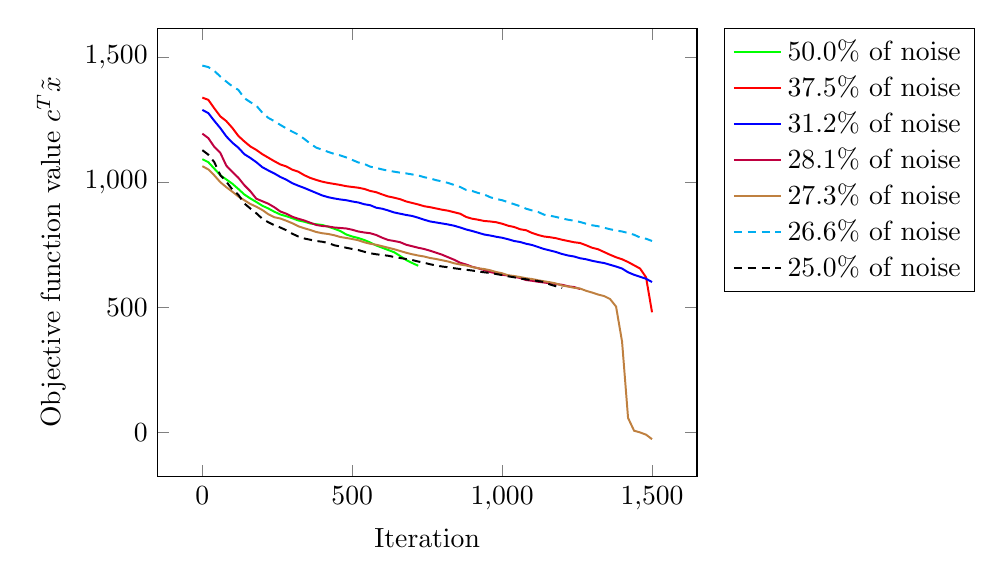
\begin{tikzpicture}
    \begin{axis}[
        legend style={
            at={(1.05,1.0)},
            anchor=north west,
            legend columns=1},
        xlabel = Iteration,
        ylabel = Objective function value $c^T \xt$,
      ]

      \addplot+[sharp plot,green,mark=none,line width=0.25mm] coordinates
        {(0,1093) (20,1081) (40,1055) (60,1029) (80,1012) (100,995) (120,974) (140,952) (160,936) (180,922) (200,907) (220,896) (240,883) (260,872) (280,865) (300,857) (320,848) (340,843) (360,836) (380,833) (400,830) (420,823) (440,815) (460,806) (480,792) (500,784) (520,778) (540,770) (560,760) (580,748) (600,739) (620,730) (640,721) (660,706) (680,690) (700,678) (720,667)

        };
      \addplot+[sharp plot,red,mark=none,line width=0.25mm] coordinates
        {(0,1339) (20,1330) (40,1296) (60,1264) (80,1245) (100,1218) (120,1186) (140,1164) (160,1144) (180,1130) (200,1113) (220,1099) (240,1085) (260,1072) (280,1064) (300,1051) (320,1043) (340,1029) (360,1018) (380,1010) (400,1003) (420,998) (440,994) (460,990) (480,985) (500,982) (520,979) (540,974) (560,966) (580,961) (600,952) (620,944) (640,939) (660,933) (680,924) (700,918) (720,912) (740,905) (760,901) (780,896) (800,891) (820,887) (840,881) (860,875) (880,862) (900,855) (920,851) (940,846) (960,844) (980,841) (1000,835) (1020,827) (1040,822) (1060,813) (1080,809) (1100,798) (1120,790) (1140,784) (1160,781) (1180,777) (1200,771) (1220,766) (1240,761) (1260,758) (1280,749) (1300,739) (1320,733) (1340,722) (1360,711) (1380,701) (1400,693) (1420,682) (1440,669) (1460,656) (1480,621) (1500,481)
        };

      \addplot+[sharp plot,blue,mark=none,line width=0.25mm] coordinates
        {(0,1290) (20,1277) (40,1246) (60,1217) (80,1184) (100,1159) (120,1139) (140,1113) (160,1098) (180,1081) (200,1061) (220,1048) (240,1036) (260,1022) (280,1011) (300,997) (320,987) (340,978) (360,968) (380,958) (400,948) (420,941) (440,936) (460,932) (480,929) (500,924) (520,920) (540,913) (560,909) (580,899) (600,895) (620,888) (640,880) (660,875) (680,870) (700,866) (720,859) (740,851) (760,844) (780,840) (800,836) (820,832) (840,827) (860,820) (880,812) (900,806) (920,799) (940,792) (960,788) (980,783) (1000,779) (1020,773) (1040,766) (1060,762) (1080,755) (1100,750) (1120,742) (1140,734) (1160,728) (1180,722) (1200,714) (1220,708) (1240,704) (1260,697) (1280,693) (1300,687) (1320,682) (1340,678) (1360,671) (1380,664) (1400,656) (1420,641) (1440,631) (1460,623) (1480,615) (1500,602)
        };

      \addplot+[sharp plot,purple,mark=none,line width=0.25mm] coordinates
        {(0,1195) (20,1177) (40,1142) (60,1118) (80,1067) (100,1042) (120,1019) (140,989) (160,965) (180,935) (200,925) (220,915) (240,901) (260,884) (280,875) (300,863) (320,855) (340,848) (360,839) (380,830) (400,826) (420,824) (440,820) (460,818) (480,816) (500,811) (520,804) (540,800) (560,797) (580,790) (600,779) (620,770) (640,766) (660,761) (680,751) (700,745) (720,739) (740,734) (760,727) (780,719) (800,711) (820,701) (840,691) (860,679) (880,672) (900,663) (920,657) (940,650) (960,642) (980,637) (1000,631) (1020,628) (1040,623) (1060,618) (1080,610) (1100,607) (1120,603) (1140,600) (1160,597) (1180,594) (1200,591) (1220,585) (1240,582) (1260,574)

        };

      \addplot+[sharp plot,brown,mark=none,line width=0.25mm] coordinates
        {(0,1065) (20,1052) (40,1028) (60,1001) (80,981) (100,963) (120,944) (140,929) (160,914) (180,903) (200,890) (220,873) (240,861) (260,856) (280,847) (300,837) (320,825) (340,817) (360,810) (380,802) (400,797) (420,794) (440,789) (460,782) (480,778) (500,774) (520,769) (540,761) (560,755) (580,751) (600,745) (620,739) (640,733) (660,726) (680,719) (700,713) (720,708) (740,704) (760,698) (780,694) (800,689) (820,684) (840,677) (860,672) (880,668) (900,662) (920,657) (940,654) (960,649) (980,642) (1000,637) (1020,629) (1040,626) (1060,622) (1080,617) (1100,614) (1120,609) (1140,605) (1160,601) (1180,596) (1200,588) (1220,584) (1240,579) (1260,576) (1280,567) (1300,560) (1320,552) (1340,546) (1360,534) (1380,504) (1400,364) (1420,59) (1440,8) (1460,1) (1480,-8) (1500,-26)
        };

      \addplot+[sharp plot,cyan,mark=none,line width=0.25mm] coordinates
        {(0,1467) (20,1461) (40,1446) (60,1423) (80,1403) (100,1384) (120,1370) (140,1337) (160,1321) (180,1307) (200,1279) (220,1258) (240,1245) (260,1230) (280,1216) (300,1203) (320,1191) (340,1174) (360,1155) (380,1139) (400,1131) (420,1122) (440,1114) (460,1108) (480,1100) (500,1090) (520,1080) (540,1074) (560,1063) (580,1058) (600,1052) (620,1047) (640,1043) (660,1039) (680,1036) (700,1032) (720,1028) (740,1021) (760,1016) (780,1009) (800,1004) (820,998) (840,990) (860,982) (880,970) (900,966) (920,958) (940,952) (960,941) (980,934) (1000,929) (1020,921) (1040,913) (1060,905) (1080,895) (1100,888) (1120,882) (1140,871) (1160,867) (1180,862) (1200,856) (1220,851) (1240,847) (1260,842) (1280,835) (1300,829) (1320,825) (1340,819) (1360,813) (1380,808) (1400,804) (1420,798) (1440,791) (1460,780) (1480,775) (1500,766)
        };


      \addplot+[sharp plot,black,mark=none,line width=0.25mm] coordinates
        {(0,1129) (20,1111) (40,1081) (60,1029) (80,1003) (100,972) (120,951) (140,916) (160,896) (180,877) (200,855) (220,841) (240,829) (260,820) (280,809) (300,795) (320,784) (340,776) (360,771) (380,766) (400,763) (420,758) (440,749) (460,744) (480,739) (500,734) (520,730) (540,723) (560,717) (580,713) (600,710) (620,707) (640,702) (660,698) (680,694) (700,690) (720,684) (740,679) (760,673) (780,668) (800,664) (820,661) (840,657) (860,654) (880,651) (900,648) (920,644) (940,641) (960,638) (980,634) (1000,630) (1020,625) (1040,621) (1060,616) (1080,613) (1100,609) (1120,606) (1140,602) (1160,592) (1180,585) (1200,578)

        };

      \legend{
        50.0\% of noise,
        37.5\% of noise,
        31.2\% of noise,
        28.1\% of noise,
        27.3\% of noise,
        26.6\% of noise,
        25.0\% of noise,
      }
    \end{axis}
  \end{tikzpicture}
  \caption[Objective function value change during Dikin's algorithm for different percent of noise]
  {Objective function value change during Dikin's algorithm for different percent of noise.
    Message is \textit{I like Jubilee cookies!},
    signal dimension factor $k=2$. The maximum percent of noise for which message was successfully restores is \textbf{27.3\%} }\label{fig:dik_multiple}
\end{figure}

\section{Q7: Integer programming}
Imposing binary (integer) variables SciPy is done via adding parameter \textit{integrality} to function \textit{scipy.optimize.linprog}. Specifically, \textit{integrality} determines for each variable whether it is integer or continuous: 0 means that parameter is continuous, 1 --- integer.

Let us for this section consider LOP in geometric form (\Cref{eq:geom}), as it is solved faster than LOP in standard form. So the integrality for $z'$ would be $w = \irow{1_p & 0_m}$, as only part of $z'$ denoting the $x$ should be restricted to be integers. Moreover, first two `row blocks' of $A'$ can be removed, and instead the \textit{bounds} parameter of \textit{scipy.optimize.linprog} can be used. The bounds would be $(0,1)$ for first $p$ coordinates of $z'$ (as $0 \leq x \leq 1$) and $(0, +\inf)$ for the last m coordinates (as $z \geq 0$). The resulting function is demonstrated on \Cref{lst:int}. Note, that the maximum running time is restricted, as it may take a lot of time to complete (especially for not short messages and high percent of noise).

The results (\Cref{fig:noise_int}) show, that introducing integer restrictions increases the maximum percent of noise up to what the messages can be decrypted. However, time complexity of optimization problem with integer constraints is \textbf{significantly higher} (up to 10 times) than without integer constraints.


\begin{figure}[hbthbt]
  \centering
  \pgfplotsset{compat=1.10}
  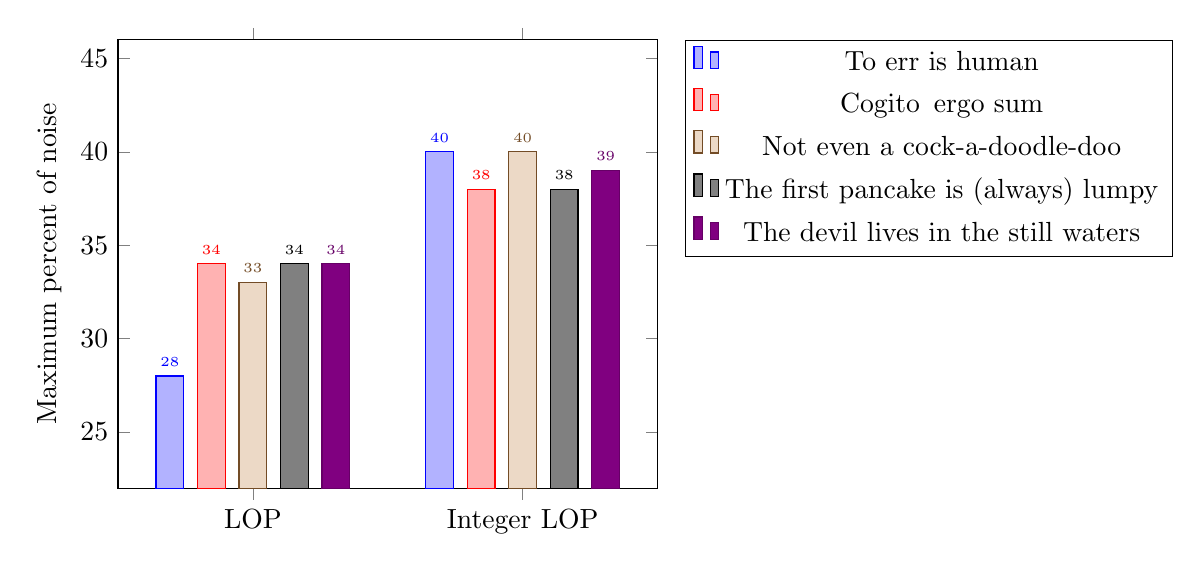
\begin{tikzpicture}
    \begin{axis}[
        ybar,
        enlargelimits=0.5,
        legend style={
            at={(1.05,1.0)},
            anchor=north west,
            legend columns=1},
        ylabel = Maximum percent of noise,
        ybar=5pt,
        symbolic x coords={LOP,Integer LOP},
        xtick=data,
        nodes near coords,
        every node near coord/.append style={font=\tiny},
        nodes near coords align={vertical},
        legend style={/tikz/every even column/.append style={row sep=0.1cm}}]
      \addplot coordinates {(LOP, 28) (Integer LOP, 40)};
      \addplot coordinates {(LOP, 34) (Integer LOP, 38)};
      \addplot coordinates {(LOP, 33) (Integer LOP, 40)};
      \addplot coordinates {(LOP, 34) (Integer LOP, 38)};
      \addplot coordinates {(LOP, 34) (Integer LOP, 39)};

      \legend{To err is human,Cogito\, ergo sum,Not even a cock-a-doodle-doo,
        The first pancake is (always) lumpy,The devil lives in the still waters}
    \end{axis}
  \end{tikzpicture}
  \caption[Maximum level of noise up to what the messages can be decrypted (signal dimension factor $k=2$)]
  {Maximum level of noise up to what the messages can be decrypted (signal dimension factor $k=2$).
    \textit{LOP} means that no integer constraints were applied to the parameters vector, and  \textit{Integer LOP} means that integer programming was applied}\label{fig:noise_int}
\end{figure}



\clearpage
\appendix

\part*{Supplementary material}
\section{Listings for Q3}


\begin{lstlisting}[language=Python, caption={Naive message decryption. The output is tuple of solution of the problem, and decrypted message itself}, label={lst:naive}]
    def extract_message_naive(encoding_matrix, noisy_signal):
      res, *_ = scipy.linalg.lstsq(a=encoding_matrix,b=noisy_signal)
      return res, res
  \end{lstlisting}




\begin{lstlisting}[language=Python, caption={Message decryption based on solution of LOP in geometric form. The output is tuple of solution of the problem, and decrypted message itself}, label={lst:geom}]
  def extract_message_geometric(encoding_matrix, noisy_signal):
    (m, p) = encoding_matrix.shape

    c = np.zeros(p+m)
    c[p : p + m] = np.ones(m)

    b = np.concat([np.zeros(p), -np.ones(p), -noisy_signal, noisy_signal])

    A = np.concat([
            np.concat([np.identity(p), np.zeros((p, m))], axis=1),
            np.concat([-np.identity(p), np.zeros((p, m))], axis=1),
            np.concat([-encoding_matrix, np.identity(m)], axis=1),
            np.concat([encoding_matrix, np.identity(m)], axis=1),
    ])

    res = scipy.optimize.linprog(c, A_ub=-A, b_ub=-b, method="highs")

    return res.x, res.x[:p]
\end{lstlisting}

% \newpage

\begin{lstlisting}[language=Python, caption={Message decryption based on solution of LOP in standard form. The output is tuple of solution of the problem, and decrypted message itself}, label={lst:std}]
  def extract_message_standard(encoding_matrix, noisy_signal):

    (m, p) = encoding_matrix.shape

    c = np.zeros(2 * p + 3 * m)
    c[p : p + m] = np.ones(m)

    b = np.concat([-np.ones(p), -noisy_signal, noisy_signal])

    A = np.concat(
        [
            np.concat(
                [
                  np.concat([-np.identity(p), np.zeros((p, m))], axis=1),
                  np.concat([-encoding_matrix, np.identity(m)], axis=1),
                  np.concat([encoding_matrix, np.identity(m),], axis=1),
                ]
            ),
            -np.identity(p + 2 * m),
        ], axis=1,
    )

    res = scipy.optimize.linprog(c, A_eq=A, b_eq=b, method="highs")

    return res.x, res.x[:p]
\end{lstlisting}




\section{Listings for Q4}


\begin{lstlisting}[language=Python, caption={Determining number of tight linear independent constraints for solution of linear problem in geometric form to ccheck whetther it it is a vertex of corresponding polyhedron}, label={lst:vertex}]
  def check_geom_solution_is_vertex(encoding_matrix: np.ndarray, noisy_signal: np.ndarray, solution: np.ndarray) -> bool:

    # In order to check, whether solution is a vertex, we need to use A and b from geometric form problem:
    (m, p) = encoding_matrix.shape
    b = np.concat([np.zeros(p), -np.ones(p), -noisy_signal, noisy_signal])

    A = np.concat(
        [
            np.concat([np.identity(p), np.zeros((p, m))], axis=1),
            np.concat([-np.identity(p), np.zeros((p, m))], axis=1),
            np.concat([-encoding_matrix, np.identity(m)], axis=1),
            np.concat([encoding_matrix, np.identity(m),], axis=1),
        ]
    )

    (M, N) = A.shape

    # Check which constraints are tight with some tolerance
    mask_sol_geom = np.isclose(A @ solution - b, 0, atol=1e-10)
    close_sol_geom = mask_sol_geom.sum()

    tight_constraints = A[mask_sol_geom]
    rank = int(np.linalg.matrix_rank(tight_constraints))

    return bool(rank >= N) # True!
\end{lstlisting}

\section{Listings for Q5}

\begin{lstlisting}[language=Python, caption={Binary search used to determine maximum level of noise up to what the message can be decrypted. \textit{extract\_fn} is either \textit{extract\_message\_geometric} or \textit{extract\_message\_standard}}, label={lst:bin}]
  for _ in range(max_iter):
      if up_bound - low_bound <eps:
          break
      current = (low_bound + up_bound)/2
      noise_custom = noisy_channel(y_custom, percent_error=current, seed=seed)

      decoded_custom, decoded_float_custom, __ =  extract_decoded_message(
          encoding_matrix_custom, noise_custom, dimensions_custom, extract_fn
      )

      if  decoded_custom == message_custom:
          low_bound = current
      else:
          up_bound = current
\end{lstlisting}


\newpage

\section{Listings for Q6}

\begin{lstlisting}[language=Python, caption={Extraction of dirty initial point for Dikin's method using standard form of linear optimization problem}, label={lst:dikin_init}]
  def get_dikin_initial_point(
      encoding_matrix: np.ndarray, noisy_signal: np.ndarray, epsilon: float
  ) -> tuple[np.ndarray, np.ndarray]:
      (m, p) = encoding_matrix.shape

      c = np.zeros(2 * p + 3 * m)
      b = np.concat([-np.ones(p), -noisy_signal, noisy_signal])
      A = np.concat([
            np.concat([
                      np.concat([-np.identity(p), np.zeros((p, m))], axis=1),
                      np.concat([-encoding_matrix, np.identity(m)], axis=1),
                      np.concat([encoding_matrix, np.identity(m)], axis=1),
                  ]),
           -np.identity(p + 2 * m)], axis=1)
      bounds = [(epsilon, None) for _ in range(2 * p + 3 * m)]

      res = scipy.optimize.linprog(c, A_eq=A, b_eq=b, bounds=bounds,
                                  method="highs")

      return res.x, res.x[:p]
\end{lstlisting}

% \newpage

\begin{lstlisting}[language=Python, caption={Message decryption based on Dikin's method. The output is tuple of solution of the problem, and decrypted message itself}, label={lst:dikin}]
  def extract_message_dikin(
      encoding_matrix: np.ndarray,
      noisy_signal: np.ndarray,
      x0: np.ndarray,
  ) -> tuple[np.ndarray, np.ndarray]:
      (m, p) = encoding_matrix.shape
      c = np.zeros(2 * p + 3 * m)
      c[p : p + m] = np.ones(m)

      A = np.concat(
          [np.concat([
                      np.concat([-np.identity(p), np.zeros((p, m))], axis=1),
                      np.concat([-encoding_matrix, np.identity(m)], axis=1),
                      np.concat([encoding_matrix, np.identity(m)], axis=1),
                  ]),
              -np.identity(p + 2 * m)], axis=1,
      )
      x = x0.copy()

      # Dikin's method
      for k in range(10):
          H = np.diag(1 / (x**2 + 1e-7))
          H_inv = np.linalg.inv(H)
          A_H_inv = A @ H_inv
          nu = -1 * np.linalg.inv(A_H_inv @ A.T) @ A_H_inv @ c

          s = -1 * H_inv @ (c + A.T @ nu)
          mu = 1 / np.sqrt(s.T @ H @ s)

          delta_x = mu * s

          x = x + delta_x

      return x, x[:p]
\end{lstlisting}

\newpage

\section{Listings for Q7}


\begin{lstlisting}[language=Python, caption={Message decryption based on solution of integer LOP in geometric form. The output is tuple of solution of the problem and decrypted message itself}, label={lst:int}]
  def extract_message_integer(encoding_matrix, noisy_signal, time_limit_s=120):
      (m, p) = encoding_matrix.shape

      c = np.zeros(p+m)
      c[p : p + m] = np.ones(m)

      integrality = np.ones(p+m) - c
      bounds = [*[(0,1) for _ in range(p)], *[(0,None) for _ in range(m)]]

      b = np.concat([ -noisy_signal, noisy_signal])

      A = np.concat(
          [
            np.concat([-encoding_matrix, np.identity(m)], axis=1),
            np.concat([encoding_matrix, np.identity(m)], axis=1),
          ]
      )

      res = scipy.optimize.linprog(c, A_ub=-A, b_ub=-b,
                        options={"maxiter": 20, "time_limit": time_limit_s},
                        method="highs",
                        integrality=integrality, bounds=bounds)

      return res.x, res.x[:p]
\end{lstlisting}




\end{document}
